\section{Theorie}
\label{sec:Theorie}

Einer elektromagnetischem Welle kann ein Poynting-Vektor zu geordnet werden. Der Betrag wird als $ \left| \vec{S}\right|  = v \epsilon \epsilon_0  \vec{E}²$  geschrieben werden.

Trifft eine ebene Lichtwelle unter dem Winkel  $\alpha$  aus dem Vakuum auf eine Grenzfläche zu einem anderen Medium, so wird ein Teil der Strahlung gebrochen $\vec{E_r}$ und der andere reflektiert $\vec{E_d}$. Es wird angenommen, dass kein Licht vom Medium absorbiert wird.


\begin{figure}
    \centering
    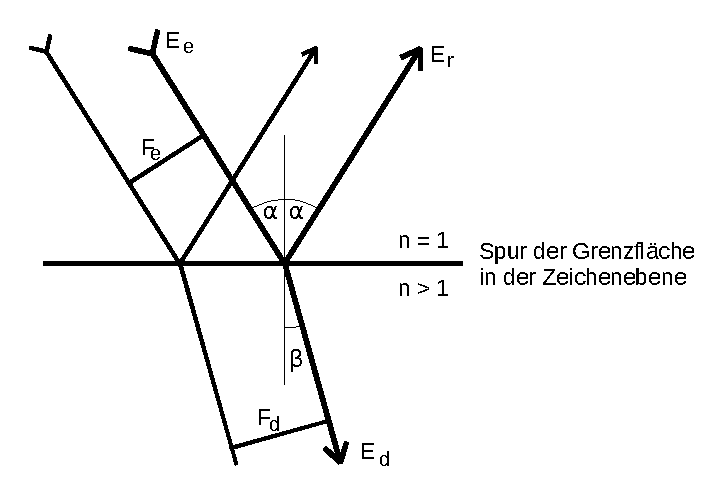
\includegraphics{Brechung an einer Ebene.pdf}
    \caption{Brechung an einer Ebene.} 
    \label{fig:abb1}
\end{figure}

Wie in der oberen Grafik \ref{fig:abb1} zu sehen ist, ist der Brechungswinkel $ \beta$ kleiner als der Brechungswinkel $\alpha$, da das Licht im Medium eine geringere Geschwindigkeit hat als im Vakuum.
Daraus bedingt sich eine Querschnittsänderung der einlaufenden Strahlung von $F_e$ auf $F_d$. 
Es gilt die Energieerhaltung, die sich als
\begin{equation}
    S_e F_e = S_r F_e +  S_d F_d
    \label{eq:Energieerhaltung}
\end{equation}
oder auch 

\begin{equation}
    S_e \cos(\alpha) = S_r \cos(\alpha) +  S_d \cos(\beta)
    \label{eq:Energieerhaltung}
\end{equation}
schreiben lässt.